% Figure M5, generated by experiments/m5_vit_cls.py.
\begin{figure}[t]
  \centering
  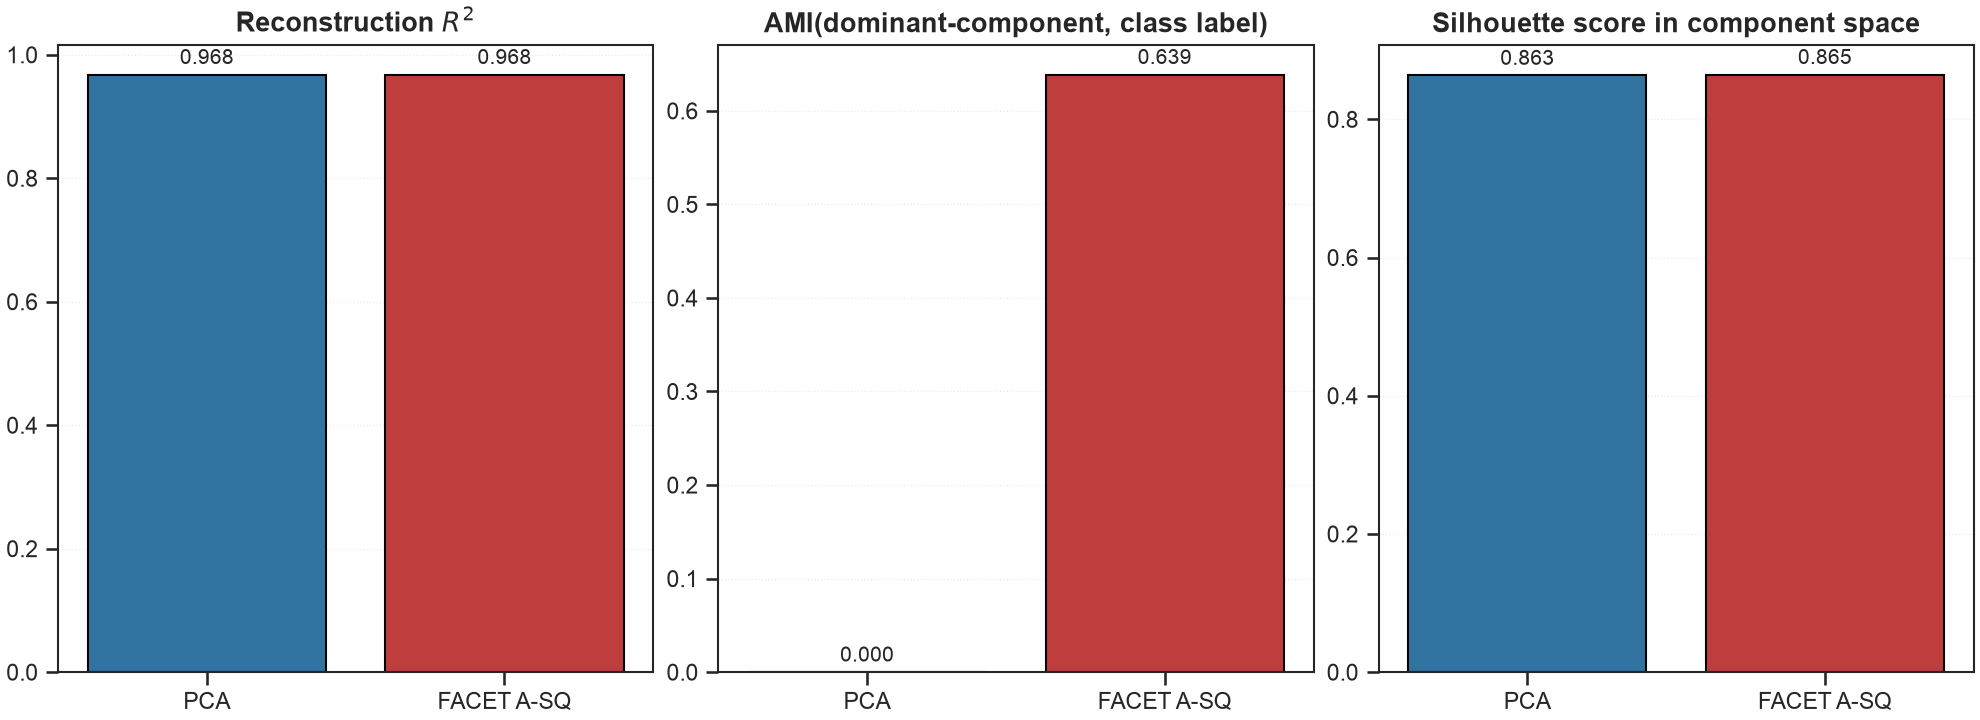
\includegraphics[width=\linewidth]{../shared/figures/generated/m5_vit_cls.png}
  \caption{\textbf{M5, ViT CLS-token decomposition on ten synthetic image classes.} Ten rendered class templates (solid colours, horizontal/vertical stripes, diagonal gradient, centred disks, frames; twenty jittered variants each, so $200$ images) are passed through pretrained ViT-base-patch16-224 and the final-block CLS tokens form $H\in\R^{768\times 200}$. FACET A-SQ and PCA fit $m{=}10$ components. \textit{Left:} reconstruction $R^2\approx 0.968$ for both methods (tied). \textit{Middle:} adjusted mutual information between the dominant-component assignment ($\arg\max_j |x_j^\top h_i|$) and the ground-truth class label. FACET: $0.64$ (strong agreement). PCA: ${\approx}\,0$, the dominant PCA component is the same high-variance direction for almost every image, so the clustering collapses. \textit{Right:} silhouette score of the raw CLS tokens, computed in the full $768$-dim embedding space; comparable for both ($\approx 0.86$). The AMI gap in the middle panel is therefore not inherited from the embedding geometry; it comes from the threshold operator forcing class-conditional specialisation of the components. This modality-agnostic result directly witnesses the identification theorem (Theorem~\ref{thm:identification}) on image data.}
  \label{fig:m5-vit-cls}
\end{figure}
